\documentclass{report}

\usepackage[utf8]{inputenc}
\usepackage[T1]{fontenc}
\usepackage[francais]{babel}
\usepackage{graphicx}
\usepackage{hyperref}
\usepackage{textcomp}
\usepackage{amsmath}
\usepackage{geometry}
\usepackage{pdfpages}

\usepackage{matlab-prettifier}

\usepackage{array,multirow,makecell}
\setcounter{secnumdepth}{3}
\setcounter{tocdepth}{3}
\setcellgapes{4pt}
\makegapedcells
\newcolumntype{R}[1]{>{\raggedleft\arraybackslash }b{#1}}
\newcolumntype{L}[1]{>{\raggedright\arraybackslash }b{#1}}
\newcolumntype{C}[1]{>{\centering\arraybackslash }b{#1}}

\usepackage[pages=some]{background}
\backgroundsetup{
	scale=1,
	color=black,
	opacity=0.1,
	angle=0,
	contents={%
		
\includegraphics[width=\paperwidth,height=\paperheight]{img/ulbback.jpg}
	}%
}


\title{\Huge\emph{Cooling Down a Coke Can}\\
	\LARGE Experiment study\\
	\vspace{11pt}
	\large Fluid Mechanics and Transport Processes}

\date{December 2015}

\author{Nathan DE PRYCK \and Miquel KEGELEIRS \and Mischa MASSON}



\begin{document}
	
	\begin{figure}[t]
		
\includegraphics[width=15cm]{img/entete.PNG}
	\end{figure}
	
	\maketitle
	
	\renewcommand{\abstractname}{``Cooling down a coke can'' \\Experiment study by Nathan De Pryck, Miquel Kegeleirs and Mischa Masson\\ Université Libre de Bruxelles\\2015-2016.}
	
	\BgThispage
	
	\begin{abstract}
		TO BE WRITTEN
	\end{abstract}
	
	\clearpage
	
	\tableofcontents
	
	\chapter{Introduction}\label{intro}
	
	This report outlines the physics behind an experiment produced during the MECA-H-3001 ``Fluid Mechanics and Transport Processes'' course of the ULB (Université Libre de Bruxelles) on Friday, the sixteenth of October 2015.
	
	The experiment can be found at \hyperref{https://www.youtube.com/watch?v=MSwc_IAPh3E}{}{}{this address}\footnote{\url{https://www.youtube.com/watch?v=MSwc_IAPh3E}} and was described as following:
	
	\begin{itemize}
		\item Three coke cans were available as well as a bucket of ice and water (at 0\textcelsius) and a drill to spin the can inside the bucket.
		\item One of the cans was used to determine the initial temperature (16\textcelsius) of the fluid (essentially water) inside the can.
		\item One can was left inside the bucket for 60 seconds and a final temperature of 11.9\textcelsius \ was measured as a result of the conductive heat transfer with the surrounding fluid.
		\item One can was spun inside the bucket for 60 seconds at about 1000 rounds per minute, and a final temperature of 11\textcelsius \ was measured as a result of the convective and conductive heat transfer.
	\end{itemize}
	
	In the first chapter, convective and conductive processes that are related to the experiment will be described. Those phenomena will then be applied to the problem via a mathematical model, including a discussion of simplifications brought to the problem in order to simplify calculations. This model will be compared to the experimental results, then a discussion on it's reliability followed by a conclusion on mathematical models in general will be presented.
	
	\chapter{Heat transfer processes}\label{htp}
	
	They are three different ways of transferring heat: conduction, convection and radiation. Due to its nature (heat exchange between two distant bodies at very different temperatures), radiation can be neglected for this experiment and will thus not be presented here.
	
	\section{Conduction}\label{cd}
	
	Thermal conduction is a heat transfer process without macroscopic movement of matter. It is initiated by a difference of temperature between contiguous bodies (or inside a body). This difference of temperature implies a difference of internal energy : the energy is higher in the warmer area than in the cooler. By diffusion and collisions between the particles, which can be molecules in a fluid or conduction electrons in a solid, particles in the warmer area transfer kinetic energy to the other particles, making them moving or vibrating faster. This creates a heat flow from the warmer area to the cooler until the system reaches thermal equilibrium. Furthermore, conduction is an irreversible process.
	
	Conduction is described by the following general equation, which is demonstrated in Professor Jean-Marie Buchlin's course\cite{Buchlin}, Chapter 13.
	
	\begin{equation}
		\frac{\delta T}{\delta t} = \bigtriangledown . (\alpha \bigtriangledown T)+ \dot{Q}_v
	\end{equation}
	
	This equation can not be used by itself because of it's nature (second degree partial derivative equation). It thus needs boundary conditions linked to properties of the system. Those can be geometrical, physical, temporal or border conditions.
	
	Boundary conditions used and simplifications of the above general equation will be discussed in chapter~\ref{mm}
		
	\section{Convection}\label{cv}
	
	Convection refers to particular heat transfers in fluids. Convection occurs when some fluid is in movement. The movement lead to an advection (heat is transported by moving matter).
	
	Convection is described as following :
	\begin{equation}
		Convection = Conduction + Advection
	\end{equation}
	
	Seeing this, it is easy to understand that convection is superior than conduction in fluids in a flux situation. 
	
	An important distinction can be made in convective heat transfers : convection can be natural or forced.
	Natural convection occurs mainly due to temperature differences which modify fluids density. Increasing the temperature amplifies thermal agitation which leads to a volume expansion along with a decreasing of density. Cold components are thus heavier and fall down while lighter hot components rise. This created a bulk fluid motion initiating a convective heat transfer called natural convection.
	Forced convection refers to a convective heat transfer due to surface forces which generates a movement in the fuid. Those surfaces forces can can be applied by either artificial ways such as fans or natural ways such as blowing wind.
	Both natural and forced convection can happend simultaneously.
	
	The flow properties also have a major impact on convective heat transfers and can be expressed through dimensionless numbers.
	As convection depends on the flow (laminar, turbulent,...), we will discuss the equation to use in the next chapter(Mathematical model, chapter~\ref{mm}).
	
	\chapter{Mathematical model}\label{mm}
	
	The idea behind mathematical models is to create a simplified version of a problem, that is accurate enough to predict the behaviour of a system, but simple enough to be resolved with few calculations.
	
	This means that some simplifications of the equations seen before can be made, using the properties of the studied system.
	
	General simplifying assumptions for the experiment will first be described and their validity will be discussed, then two simplified models will be presented: one for the non-spinning can and one for the spinning can.
	
	\section{General simplifying assumptions}\label{gsa}
	
	The first assumption that will be considered is that the fluid contained in the can has properties similar to water. Coke is indeed an aqueous solution containing sugar and other ingredients, but at relatively low concentrations.
	Properties of water can be found in annex~\ref{WTPP} and are extracted from \emph{``Perry’s Chemical Engineers’ Handbook''\cite{properties}}.
	
	Another assumption is that the can is a perfect cylinder with an height of $h=116mm$ and a diameter of $d=66mm$\footnote{dimensions are standard ones for European Aluminium $330ml$ cans, those can be found on \hyperref{http://www.webpackaging.com/en/portals/rexam/assets/11059498/spec-alu-202/}{}{}{webpackaging.com}}. In the reality, the shape of a can is a bit different to support pressure but difference should not be significant in present calculations. The material used for cans is Aluminium and since it is extremely thin(less than $1mm$) and has an excellent thermal conductivity ($>200\frac{W}{K.m}$), its influence on heat transfers can be neglected. The considered model will thus be a cylinder of water laid under water maintained at another temperature and without any matter exchange, as shown in figure~\ref{cyl}.
	
	\begin{figure}
		\label{cyl}
		\centering
		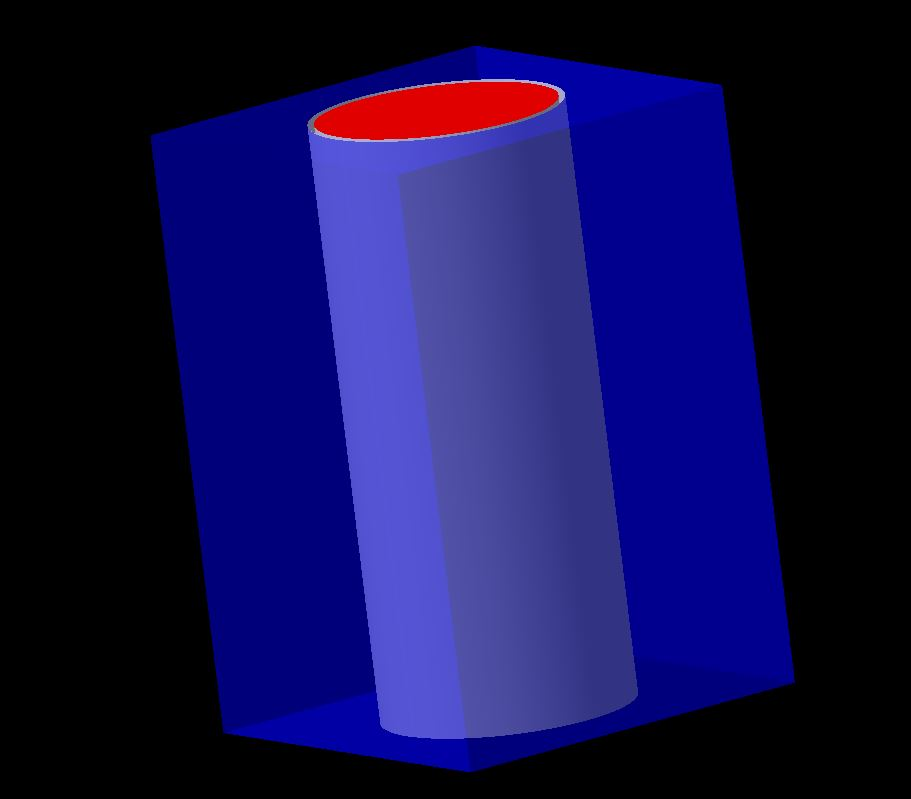
\includegraphics[width=.5\textwidth]{img/cyl.jpg}
		\caption{The red cylinder is hotter water, the blue box is colder water. No matter exchanges, only heat transfer.}
	\end{figure}
	
	Furthermore, the hypothesis that all heat exchanges between the can and surrounding ice-cold water take place on de sides of the can and not on it's top or bottom will be assumed. The total surface of the can is given by:
	
	\begin{equation}
	\begin{gathered}
		Surface= 2.Surface_{circle} + Surface_{rectangular side} \\
		\Leftrightarrow S= 2 (\pi  (\frac{d}{2})^2) + \pi dh \\
		\Leftrightarrow S= 30.8944 cm^3
	\end{gathered}
	\end{equation}
	
	Bottom and top circular surfaces have a total surface of $2xSurface_{circle}=2 (\pi  (\frac{d}{2})^2)= 6.8424 cm^3$, this is thus about $22.14\% $ of total surface. Reason why it was decided to ignore such a large portion of the can's area is because half of it is not even in contact with ice during the experiment (the system holding the can covers it's top and non-spinning can is not totally in ice), reducing the area to consider at about $11\% $ of total exchange area. This can still be seen as a large percentage, but as it is on the bottom of the can and as we are trying to cool down a liquid, the liquid in contact with the bottom part will be cooler, making heat transfer far less efficient there because cold fluids tend to be more dense than hot fluids.
	
	The last general simplification made for this experiment is to consider the mix of ice and water surrounding the can as a continuous layer of water maintained at 0\textcelsius. This should be correct enough considering that there is a large quantity of melting ice in an isolated box; and as liquid water is more flexible than ice, the can has a larger surface in contact with molten ice (and thus water) than with ice itself.
	
	
	\section{Simplified models}\label{sm}
	
	With these four simplifications in mind, two models will now be build, one for the non-spinning can and one for the spinning can.
	
	\subsection{Non-spinning can}\label{nrc}
	
	Heat transfer processes in presence are conduction and natural convection. Natural convection appears because of the density change of fluid related to temperature: the cooler the fluid, the denser it is. There is no forced convection because there is no flux in the fluid.
	
	The convective heat transfer coefficient for natural convection (in the can) is given by:
	\begin{equation}
		h_x=Ra^\alpha = cGr^\alpha Pr^\alpha
	\end{equation}
	
	Where $Gr$ is the Grashof number and $Pr$ the Prandtl number. Prandtl can be found in annex~\ref{WTPP}: water being at 16\textcelsius (about $290K$), it gives $Pr=7.56$.\\
	Grashof number is calculated using the following formula (taken from annex~\ref{FORMU}):
	\begin{equation}
	Gr=\frac{\beta g \Delta T_{ref} d^3}{\nu^2}
	\end{equation}
	
	Where:
	\begin{itemize}
		\item $\beta$ is the volume expansion coefficient, given by $\frac{1}{\rho}\frac{\delta\rho}{\delta T}$. Using the tables in annex~\ref{WTPP}, the following approximation can be made : $\beta=1.001\times 10^{-3}\frac{\frac{1}{1.000\times 10^{-3}}-\frac{1}{1.001\times 10^{-3}}}{5}=1.998\times 10^{-4} K^{-1}$.
		\item $g=9.81\frac{m^2}{s}$ is gravity.
		\item $\Delta T_{ref}=16-0=16$\textcelsius\ is the difference of temperature between the water inside the can and the ice-cold water outside of it.
		\item $d=33\times 10^{-3}m$ is the diameter of the cylinder.
		\item $\nu=\frac{\mu}{\rho}=\frac{1080\times 10^{-6}}{\frac{1}{1.001\times 10^{-3}}}=1.081\times 10^{-6}\frac{m^2}{s}$ is water's kinematic viscosity.
	\end{itemize}
	All values used come from annex~\ref{WTPP}.
	
	
	Rayleigh number is thus: 
	\begin{equation}
		Ra = GrPr= 7.56\times \frac{1.998\times 10^{-4}\times 9.81\times 16\times (66\times 10^{-3})^3}{(1.081\times 10^{-6})^2}= 5.8329\times 10^{7}
	\end{equation}
	Since $Ra<10^9$, the laminar case should be considered. Assuming that the ice-cold water around the can is at a constant temperature, it is now needed to determine which equation to use for Nusselt number.
	
	The easiest approximation is to describe the cylinder as a rectangular enclosure, with H (the height of the enclosure) equal to $h=116mm$ and L (the characteristic length of the enclosure) equal to $\frac{d}{2}=33mm$. This gives an H on L ratio of $\frac{H}{L}=3.352$. The equation 9-53 at page 555 of ``Heat and Mass Transfer: Fundamentals and Applications''~\cite{HaMT}, chapter 9-5 will thus be used:
	\begin{equation}
		\begin{gathered}
		Nu=0.22(\frac{Pr}{0.2+Pr}Ra)^{0.28}(\frac{H}{L})^{-1/4}\\
		\Leftrightarrow Nu=2.3835\times 10^{1}
		\end{gathered}	
	\end{equation}
	and:
	\begin{equation}
		\begin{gathered}
		Nu=\frac{hL}{k}\\
		\Leftrightarrow h=\frac{Nu k}{L}=\frac{2Nu k}{d}\\
		\Leftrightarrow h=4.3191\times 10^2 \frac{W}{m^2K}
		\end{gathered}	
	\end{equation}
	
	Biot number is given by $Bi=\frac{hL}{k}=\frac{hd}{2k}=23.8347 > 1$. This indicates that \emph{the system can not be considered as a Lumped system}, the temperature inside the can is not homogeneous. But, as the temperature is measured manually by putting a thermometer inside the can, and as the size of the thermometer is not negligible compared to the small radius of the can, the system will be simplified by using the equations for a Lumped system in the case of sensible heat transfer:
	
	\begin{equation}
		\begin{gathered}
		\rho CV\frac{dT}{dt}=-hS_{tot}(T-T_{ext})\\
		\Leftrightarrow \frac{hS_{tot}}{\rho CV}dt=\frac{1}{(T_{ext}-T)}dT\\
		\Leftrightarrow \frac{4h}{\rho Cd}dt=\frac{1}{(T_{ext}-T)}dT\\
		\Leftrightarrow \frac{4h}{\rho Cd}t=ln(\frac{T_0-T_{ext}}{T_f-T_{ext}})\\
		\Leftrightarrow e^{\frac{4h}{\rho Cd}t}=\frac{T_0-T_{ext}}{T_f-T_{ext}}\\
		\Leftrightarrow T_f=T_{ext}+\frac{T_0-T_{ext}}{e^{\frac{4h}{\rho Cd}t}}
		\end{gathered}
	\end{equation}
	
	This, when using the parameters of the experiment, would have given $T_f=284.14K=10.99$\textcelsius\ after $t=60s$.
	
	This value is quite far from what is observed in the experiment. This is due to some simplifications made here, like, for example, using the Lumped system equations, or some of the parameters choice.
	
	Looking at the parameters, the approximation made for $\beta$ can be refined if, instead of using the value approximated over the temperature interval, the value for $\beta$ at 15\textcelsius\ given in Appendix A-1, table A-9 of ``Heat and Mass Transfer: Fundamentals and Applications''~\cite{HaMT}: $\beta=1.38\times 10^{-4} K^{-1}$ is used. Injecting this in the model already adds some accuracy, with a temperature of $11.40$\textcelsius\ ($284.55K$).
	
	Moreover, the values of $\beta$ and $Pr$ are not fixed, they depend on temperature. To get even more accurate results, ``mean values'' of those two numbers will now be taken. In order to do so, since their evolution is small in the interval of temperatures ($1.38\times 10^{-4}$ to $0.733\times 10^{-4}$ for $\beta$ and $8.09$ to $9.45\times 10^{-4}$ for Prandtl~\footnote{Be warned that the values for Prandtl are different than the one used before: this is due to the fact it was decided to use values from the same source (``Heat and Mass Transfer: Fundamentals and Applications''~\cite{HaMT}) here to ensure they are calculated the same way. This also shows the differences that can be observed for the same number, depending of the source and the temperatures it uses as standards}), the assumption is made that their variation is linear and that the linear mean value on the interval can be used. In the end, it gives $\beta=1.056\times 10^{-4} K^{-1}$ and $Pr=8.77$.
	
	Those corrections, when injected in the model, give $T_f=284.68K=11.53$\textcelsius\ after $t=60s$. This value seems acceptable, considering the simplifications made on the system. The error compared to the experimental results is about $3.11$\textdiscount, and the fact that the temperature measurement made during the experiment where not immediate and that the thermometer itself was warm has to be taken in account.
	
	The code used for this part of the model can be found in annex~\ref{codeNS}
	
	
	Graph~\ref{NSg} gives the evolution of temperature($K$) with time($s$) for the last model with enhanced approximations of Prandtl and $\beta$.
	\begin{figure}
		\label{NSg}
		\centering
		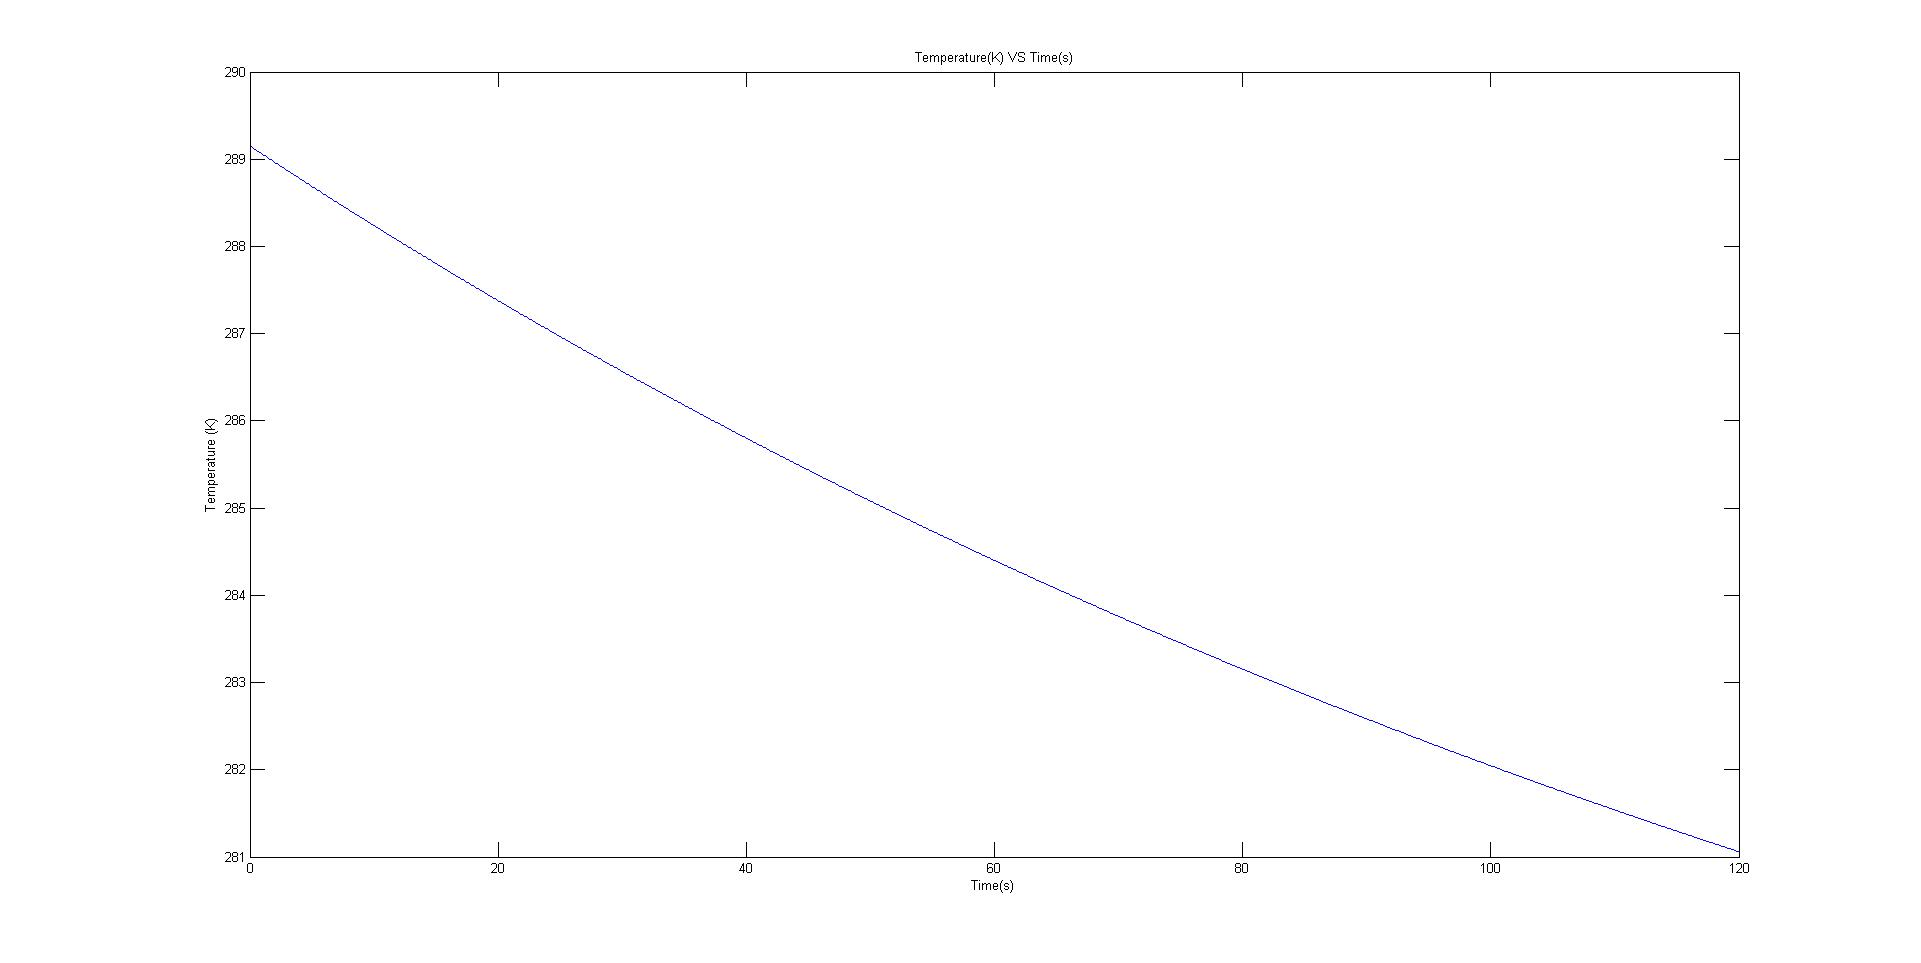
\includegraphics[width=\textwidth]{img/NSg.jpg}
	\end{figure}
	
	
	
	\subsection{Spinning can}
	
	\chapter[Reality and mathematical model]{Comparison between reality and the mathematical model}\label{rvmm}
	
	\chapter{Conclusion}\label{ccl}
	
	
	\appendix
	
	\chapter{Water Thermo-Physical Properties}\label{WTPP}
	
	These chart can be are extracted from ``Perry’s	Chemical Engineers’ Handbook'', Chapter 2\cite{properties}.
	
	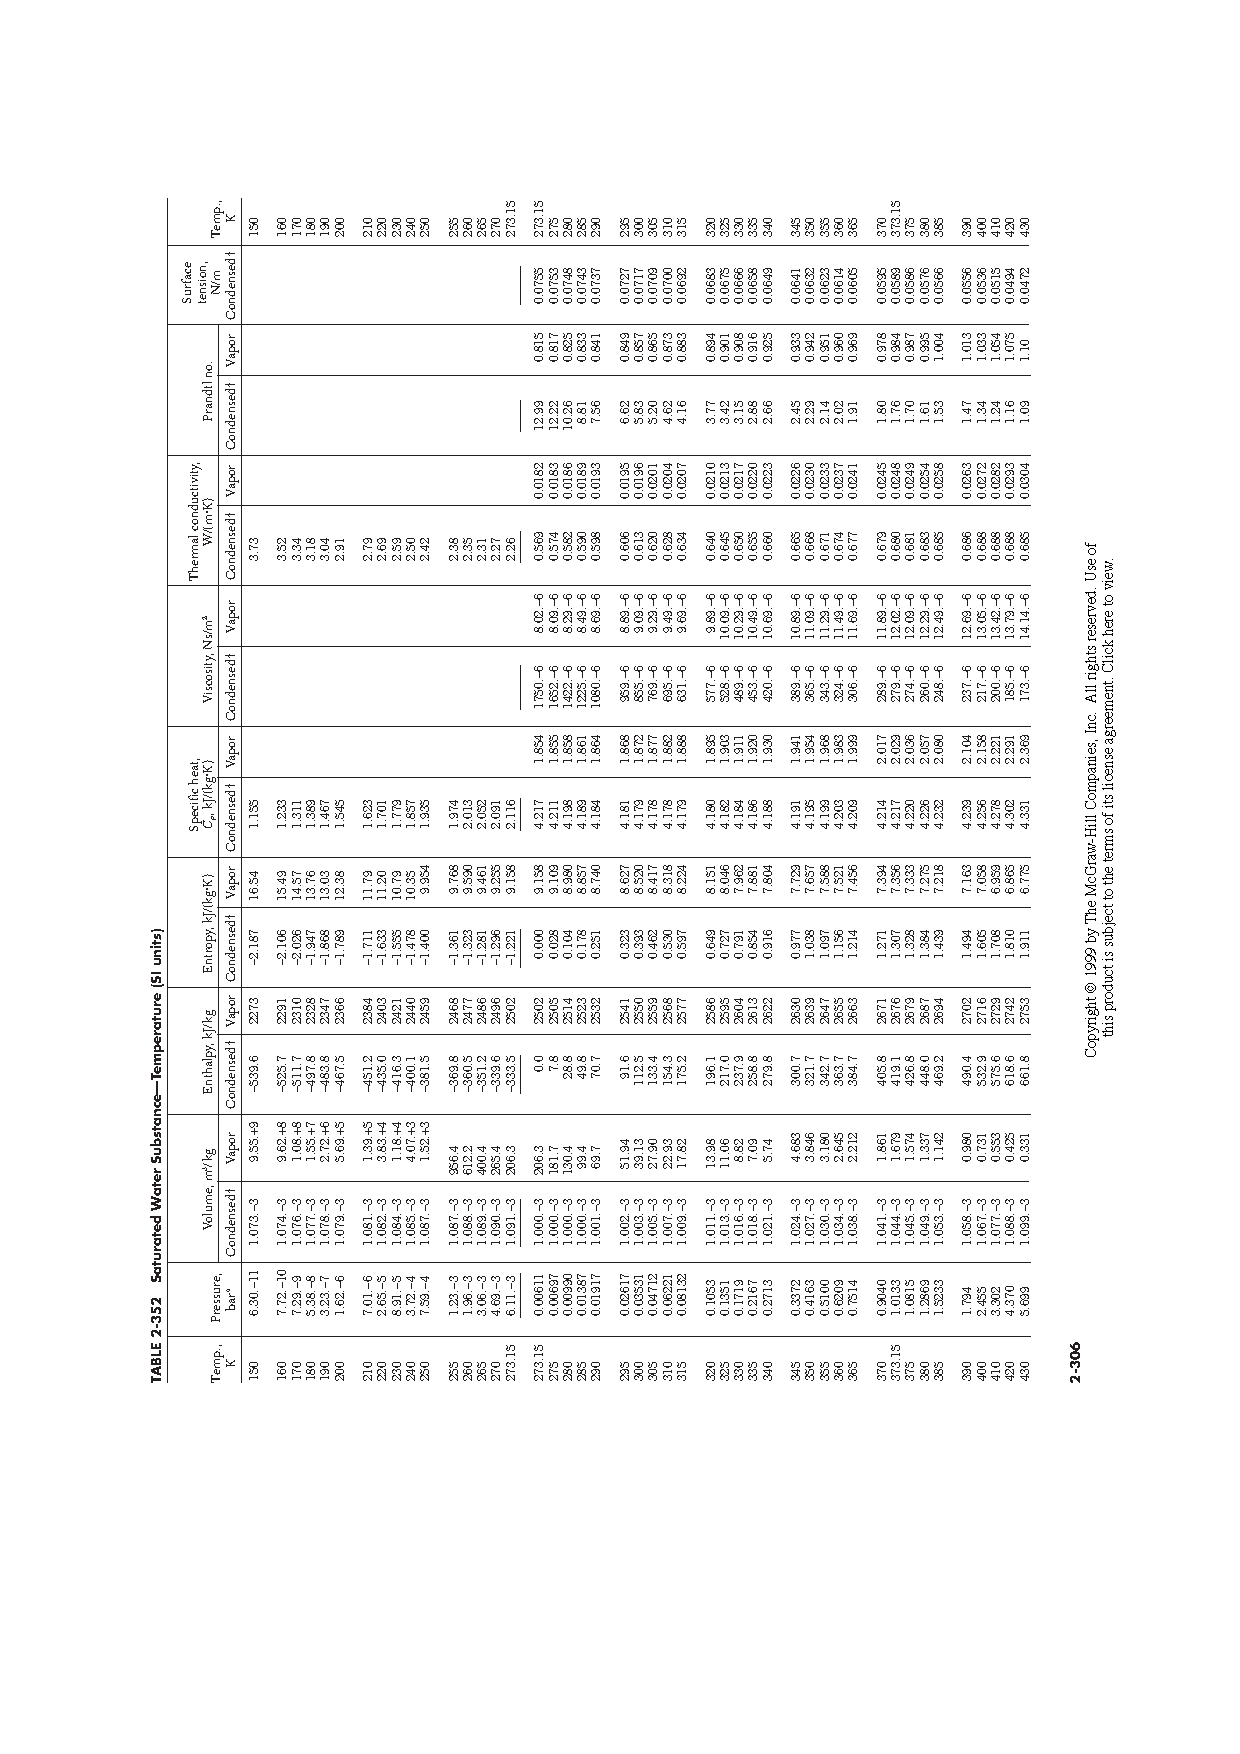
\includepdf[pages={-}]{WaterThermo-PhysicalProperties.pdf}
	
	\chapter{Formula Sheet}\label{FORMU}
	
	The following formula sheet was given and demonstrated at Pr. Parente's course ``MECA-H3001: Fluid mechanics and transfer processes''.
	
	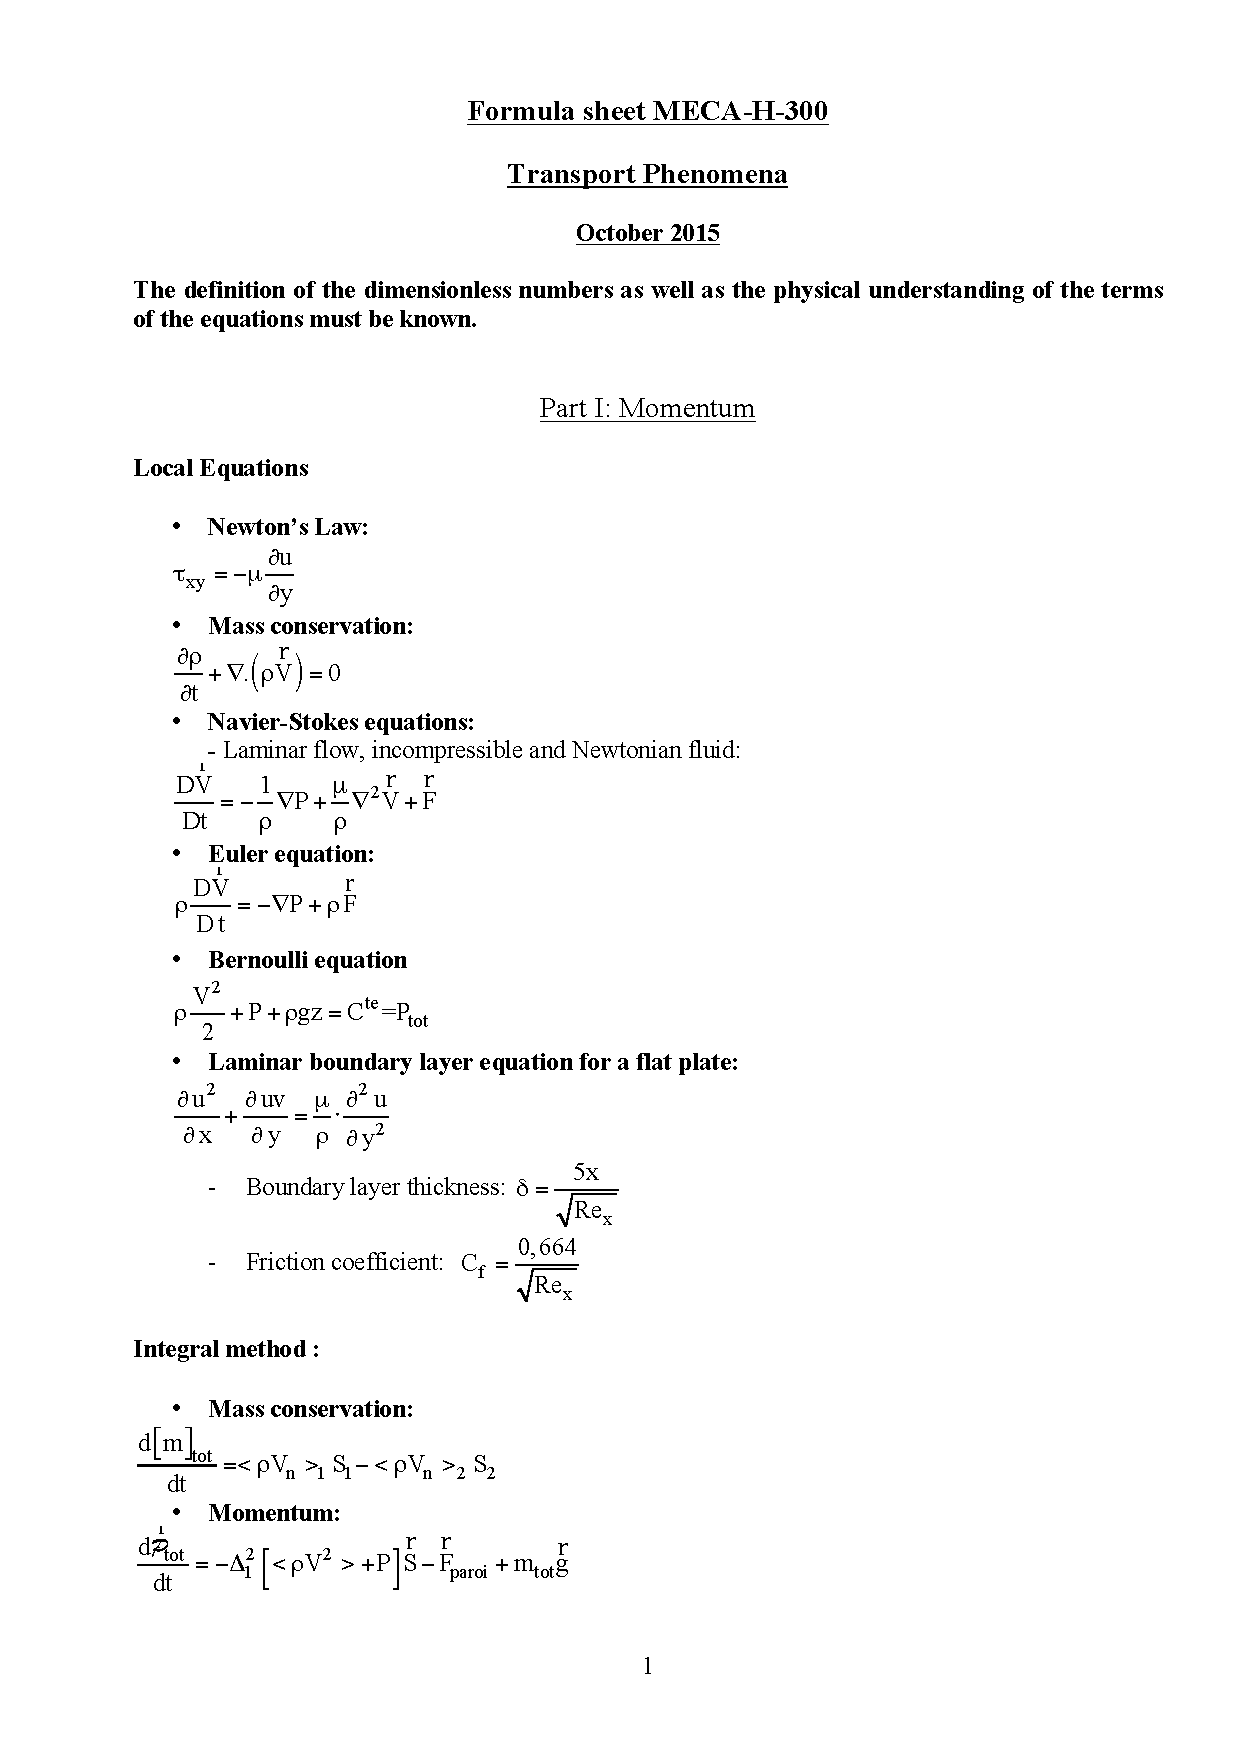
\includepdf[pages={-}]{FormulaSheet.pdf}
	
	\chapter{Codes}
	
	The following codes where used to calculate the models and obtain the different graphs. The reader should be advised this code is only usable for this work and should not be reused as it takes in account parameters and simplifying assumptions made for this particular experiment.
	
	\section{Non-spinning model}\label{codeNS}
	
	\begin{lstlisting}[style=Matlab-editor]
	t = linspace(0,120,1210);
	Pr=8.77
	beta=1.056*10^(-4)
	Ra=Pr*(beta*9.81*16*(.066)^(3))/(1.081*10^(-6))^2
	Nu=0.22*(Pr*Ra/(0.2+Pr))^(0.28) *(0.116/0.033)^(-1/4)
	h=Nu*0.598/.033
	T60=(16./(exp((4*h*60)/(1000*4184*.066))))
	Tf=273.15 +(16./(exp((4*h*t)/(1000*4184*.066))));
	plot(t,Tf,60,T60+273.15,'*')
	strValues = num2str([60 T60+273.15]);
	text(60,T60+273.15,strcat('(',strValues,')'),'VerticalAlignment','bottom');
	title('Temperature(K) VS Time(s)')
	xlabel('Time(s)')
	ylabel('Temperature (K)')
	\end{lstlisting}
	
	
	\bibliography{biblio}{}
	\bibliographystyle{plain}
	
\end{document}